\documentclass[aspectratio=169]{beamer}
\usepackage{beamerstyle}

\begin{document}

\begin{frame}
	\vspace{2cm}
	\begin{center}
		{\Huge\textbf{\textcolor{copenhagenred}{Unbiased MCMC}}}
		\vspace{1cm}

		\rule{4cm}{3pt}
		\vspace{2cm}
	\end{center}
\end{frame}

\begin{frame}
	\frametitle{Unbiased MCMC}

	\begin{itemize}
		\item Standard MCMC estimators are biased for any fixed number of iterations.
		\item We do not know in practice how many iterations are needed to reduce bias to an acceptable level.
		\item Burn-in period is often used to reduce bias, but it is difficult to choose appropriately.
		\item Unbiased MCMC estimators can be constructed using coupling techniques.
		\item Glynn--Rhee estimator provides a way to obtain unbiased estimates of expectations with respect to the target distribution.
		\item Key assumptions include moment conditions, geometric tail bounds on meeting times, and the property that chains stay together after meeting.
		\item Since the estimator is unbiased, we can generate shorter chains (in parallel) and average them to reduce variance without introducing bias.
		\item The cost is more complexity in implementation and the need to design effective coupling strategies.
	\end{itemize}
\end{frame}

% First slide
\begin{frame}
	\frametitle{Unbiased MCMC}

	\begin{itemize}
		\item \textbf{Unbiased estimation using coupling} (Glynn and Rhee, 2014, Jacob et al., 2020 \& 2024)

		      \begin{align*}
			      X_0            & \sim \pi_0, \quad Y_0 \sim \pi_0, \quad X_1 \sim K(X_0, \cdot)       \\
			      (X_{t+1}, Y_t) & \sim \bar{K}((X_t, Y_{t-1}), (\cdot, \cdot)), \quad \forall t \geq 1
		      \end{align*}

		\item \textbf{Assumption 1}: $E_\pi[h(X)] = \lim_{t \to \infty} E[h(X_t)]$ and there is $\eta > 0$ and $D < \infty$ that $E[|h(X_t)|^{2+\eta}] \leq D$ for all $t$.

		\item \textbf{Assumption 2}: meeting/coupling time
		      \[
			      \tau = \inf\{t \geq 1 : X_t = Y_{t-1}\} \text{ satisfies } \Pr(\tau > t) \leq C\delta^t \text{ for all}
		      \]
		      $t$, for some constant $C < \infty$ and $\delta < 1$.

		\item \textbf{Assumption 3}: the chains stay together after meeting: $X_t = Y_{t-1}$ for all $t \geq \tau$.

	\end{itemize}

\end{frame}

\begin{frame}
	\frametitle{Glynn--Rhee estimator - assumptions}
	\begin{itemize}
		\item \textbf{Assumption 1}: To ensure existence of moments
		\item \textbf{Assumption 2}: This is the hardest to verify in practice. It requires the coupling to be efficient enough so that the meeting time has geometric tails
		\item \textbf{Assumption 3}: This is often easy to ensure in practice by designing the coupling appropriately
	\end{itemize}
\end{frame}


\begin{frame}
	\frametitle{Glynn--Rhee debiasing formula}
	\begin{theorem}
		Under assumptions A1-A3, for any fixed $k \geq 0$

		\[
			E_\pi[h(X)]  =E[h(X_k) + \sum_{t=k+1}^{\tau-1} [h(X_t) - h(Y_{t-1})] ]
		\]
	\end{theorem}

	\begin{align*}
		 & E_\pi[h(X)] \underset{\text{by A1}}{=} \lim_{t \to \infty} E[h(X_t)] = E[h(X_k)] + \sum_{t=k+1}^{\infty} \{E[h(X_t)] - E[h(X_{t-1})]\} \\
		 & \underset{\text{by A1 and A2}}{=} E\left[h(X_k) + \sum_{t=k+1}^{\infty} [h(X_t) - h(\textcolor{red}{Y_{t-1}})]\right]
		\underset{\text{by A3}}{=} E\left[h(X_k) + \sum_{t=k+1}^{\textcolor{red}{\tau-1}} [h(X_t) - h(Y_{t-1})]\right]
	\end{align*}

\end{frame}

\begin{frame}
	\frametitle{Example of Coupling: Maximal Coupling}
	\begin{algorithm}[H]
		\caption{Sampling a coupling of $p$ and $q$. The coupling maximizes $\mathbb{P}(X = Y)$.}
		\begin{algorithmic}[1]
			\STATE Sample $X \sim p$.
			\STATE Sample $U \sim \text{Uniform}(0, 1)$.
			\IF {$U \leq q(X)/p(X)$}
			\STATE set $Y = X$.
			\ELSE
			\WHILE {true}
			\STATE sample $Y^* \sim q$ and $W^* \sim \text{Uniform}(0, 1)$ until $W^* > p(Y^*)/q(Y^*)$
			\ENDWHILE
			\STATE set $Y = Y^*$.
			\ENDIF
			\STATE Return $(X, Y)$.
		\end{algorithmic}
	\end{algorithm}
\end{frame}

\begin{frame}
	\frametitle{Maximal Coupling of two Gaussians}
	\begin{figure}[h]
		\centering
		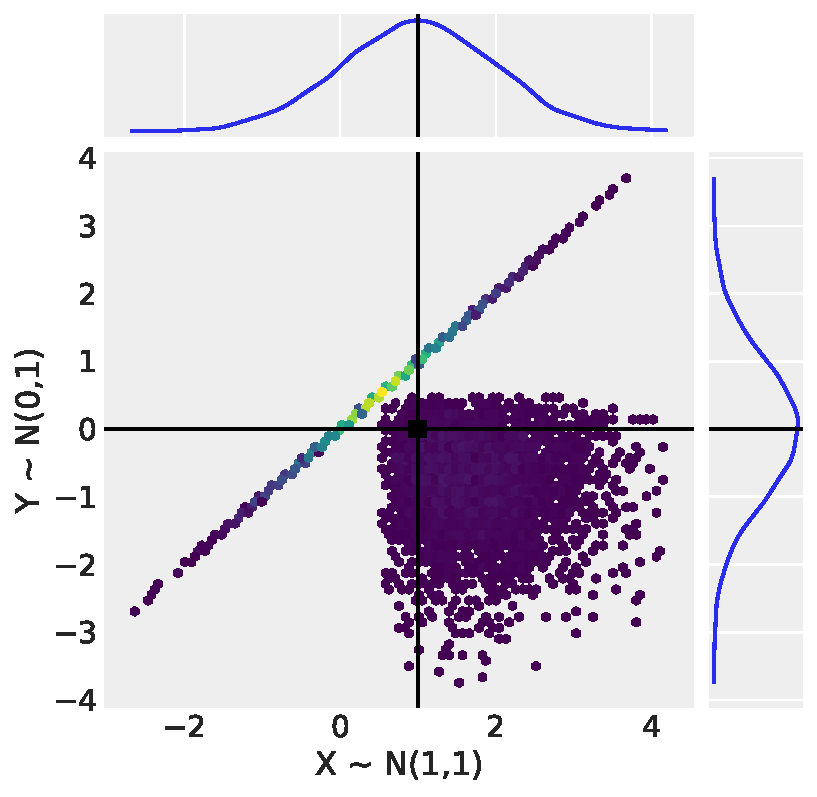
\includegraphics[width=0.4\textwidth]{maximal_coupling_plot.pdf}
		\caption{Maximal coupling of $\mathcal{N}(0, 1)$ and $\mathcal{N}(1, 1)$. Geometric interpretation: Maximizes mass on the diagonal.}
	\end{figure}
\end{frame}


\begin{frame}
	\frametitle{Coupling}
	Couplings of MCMC algorithms can be devised using maximal couplings, reflection couplings, and
	common random numbers. We have focused on couplings that can be implemented without further
	analytical knowledge about the target distribution or about the MCMC kernels. However, these couplings
	might result in prohibitively large meeting times, either because the marginal chains mix slowly
	or because the coupling strategy is ineffective
\end{frame}









\begin{frame}
	\frametitle{Coupling}
	\begin{algorithm}[H]
		\caption{Successful coupling of chains with lag $L$ and length $\ell$. Coupled initial distribution: $\tilde{\pi}_0$, transition: $P$, coupled transition: $\tilde{P}$, meeting time $\tau = \inf\{t \geq L : X_t = Y_{t-L}\}$.}
		\begin{algorithmic}[1]
			\STATE Sample $(X_0, Y_0)$ from $\tilde{\pi}_0$.
			\IF {$L \geq 1$}
			\FOR {$t = 1, \ldots, L$}
			\STATE sample $X_t$ from $P(X_{t-1}, \cdot)$
			\ENDFOR
			\ENDIF
			\FOR {$t \geq L$}
			\WHILE {true}
			\STATE sample $(X_{t+1}, Y_{t-L+1})$ from $\tilde{P}((X_t, Y_{t-L}), \cdot)$ until $X_{t+1} = Y_{t-L+1}$ and $t + 1 \geq \ell$
			\ENDWHILE
			\ENDFOR
			% \STATE If $L \geq 1$, for $t = 1, \ldots, L$, sample $X_t$ from $P(X_{t-1}, \cdot)$.
			% \STATE For $t \geq L$, sample $(X_{t+1}, Y_{t-L+1})$ from $\tilde{P}((X_t, Y_{t-L}), \cdot)$ until $X_{t+1} = Y_{t-L+1}$ and $t + 1 \geq \ell$.
		\end{algorithmic}
	\end{algorithm}
\end{frame}


\end{document}